\documentclass[notheorems]{beamer}
\usetheme[secheader]{Lab2C}
%\usetheme{Lab2C} % disable pgf drawing to speed up compilation in development
\usepackage{graphicx}
\usepackage{array}
\usepackage{subcaption}
\usepackage{listings}
\usepackage{color}
\usepackage{algorithmic}
\usepackage{amssymb}
\usepackage[square,sort,comma,numbers]{natbib}
\usepackage{amsfonts}
\usepackage{amsmath}
\usepackage{amssymb}
\usepackage{amsthm}
\usepackage{algorithm}
\usepackage{algorithmic}
\usepackage{bm}
\usepackage{hyperref}
\usepackage{footmisc}
\usepackage{xcolor}




\DeclareMathOperator*{\argmin}{arg\,min}
\DeclareMathOperator*{\argmax}{arg\,max}
\DeclareMathOperator\E{\mathbb{E}}
\DeclareMathOperator\Var{\mathrm{Var}}
\def\R{\mathbb{R}}
\def\P{\mathcal{P}}
\usepackage{mathtools}
\DeclarePairedDelimiter\abs{\lvert}{\rvert}
\DeclarePairedDelimiter\norm{\lVert}{\rVert}
\DeclarePairedDelimiter\inner{\langle}{\rangle}
\DeclarePairedDelimiter\floor{\lfloor}{\rfloor}
\DeclarePairedDelimiter\ceil{\lceil}{\rceil}
\def\red#1{\textcolor{red}{#1}}
\makeatletter
\newcommand{\algorithmicfunction}{\textbf{function}}
\newcommand{\algorithmicendfunction}{\algorithmicend\ \algorithmicfunction}
\newenvironment{ALC@func}{\begin{ALC@g}}{\end{ALC@g}}
\newcommand{\FUNCTION}[2][default]{\ALC@it\algorithmicfunction\ #2\ %
\textbf{:}%
\ALC@com{#1}\begin{ALC@func}}
\ifthenelse{\boolean{ALC@noend}}{
    \newcommand{\ENDFUNCTION}{\end{ALC@func}}
  }{
    \newcommand{\ENDFUNCTION}{\end{ALC@func}\ALC@it\algorithmicendfunction}
  }
\makeatother
\theoremstyle{definition}
\newtheorem{definition}{Definition}
\newtheorem{theorem}{Theorem}
\newtheorem{example}{Example}
\newtheorem{proposition}{Proposition}
\newtheorem{corollary}{Corollary}
\newtheorem{lemma}{Lemma}
\newtheorem{remark}{Remark}

\DeclareMathOperator{\Bern}{Bern}
\newcommand\independent{\protect\mathpalette{\protect\independenT}{\perp}}
\def\independenT#1#2{\mathrel{\rlap{$#1#2$}\mkern2mu{#1#2}}}

\definecolor{mygray}{rgb}{0.5,0.5,0.5}
\lstset{
numbers=left,
numbersep=5pt,
numberstyle=\tiny\color{mygray}
}

\newif\ifbeamer
\beamertrue
%\setbeamertemplate{footline}[frame number]
%\logo{\includegraphics[height=0.8cm]{ieee_logo.eps}}
\title[Error Rate of Stochastic Block Model with Symmetric Side Information]{On the Optimal Error Rate of Stochastic Block Model with Symmetric Side Information}
\author{Feng Zhao\inst{1}}
\institute{\inst{1}Dept. of Electronic Engineering, Tsinghua University, 2017-present
\and\inst{2}Department of Electrical Engineering, California Institute of Technology
	\\ \vskip 0.5cm Noah Group Interview 2021}
\date{\today}
\begin{document}
\begin{frame}
	\titlepage
\end{frame}
%\section*{Outline}
\begin{frame}
	\tableofcontents
\end{frame}
\section{Background}
\subsection{Community Detection}
\begin{frame}{Community Detection}
	\begin{columns}
		\column{0.5\textwidth}
		\begin{figure}
			
\includegraphics[width=0.8\textwidth]{cd.png}
		\end{figure}
	\column{0.5\textwidth}
	Community Detection is inferring the group of vertices which are more
	densely connected in a graph
	\end{columns}
	\begin{columns}
		\column{0.33\textwidth}
		\begin{figure}
			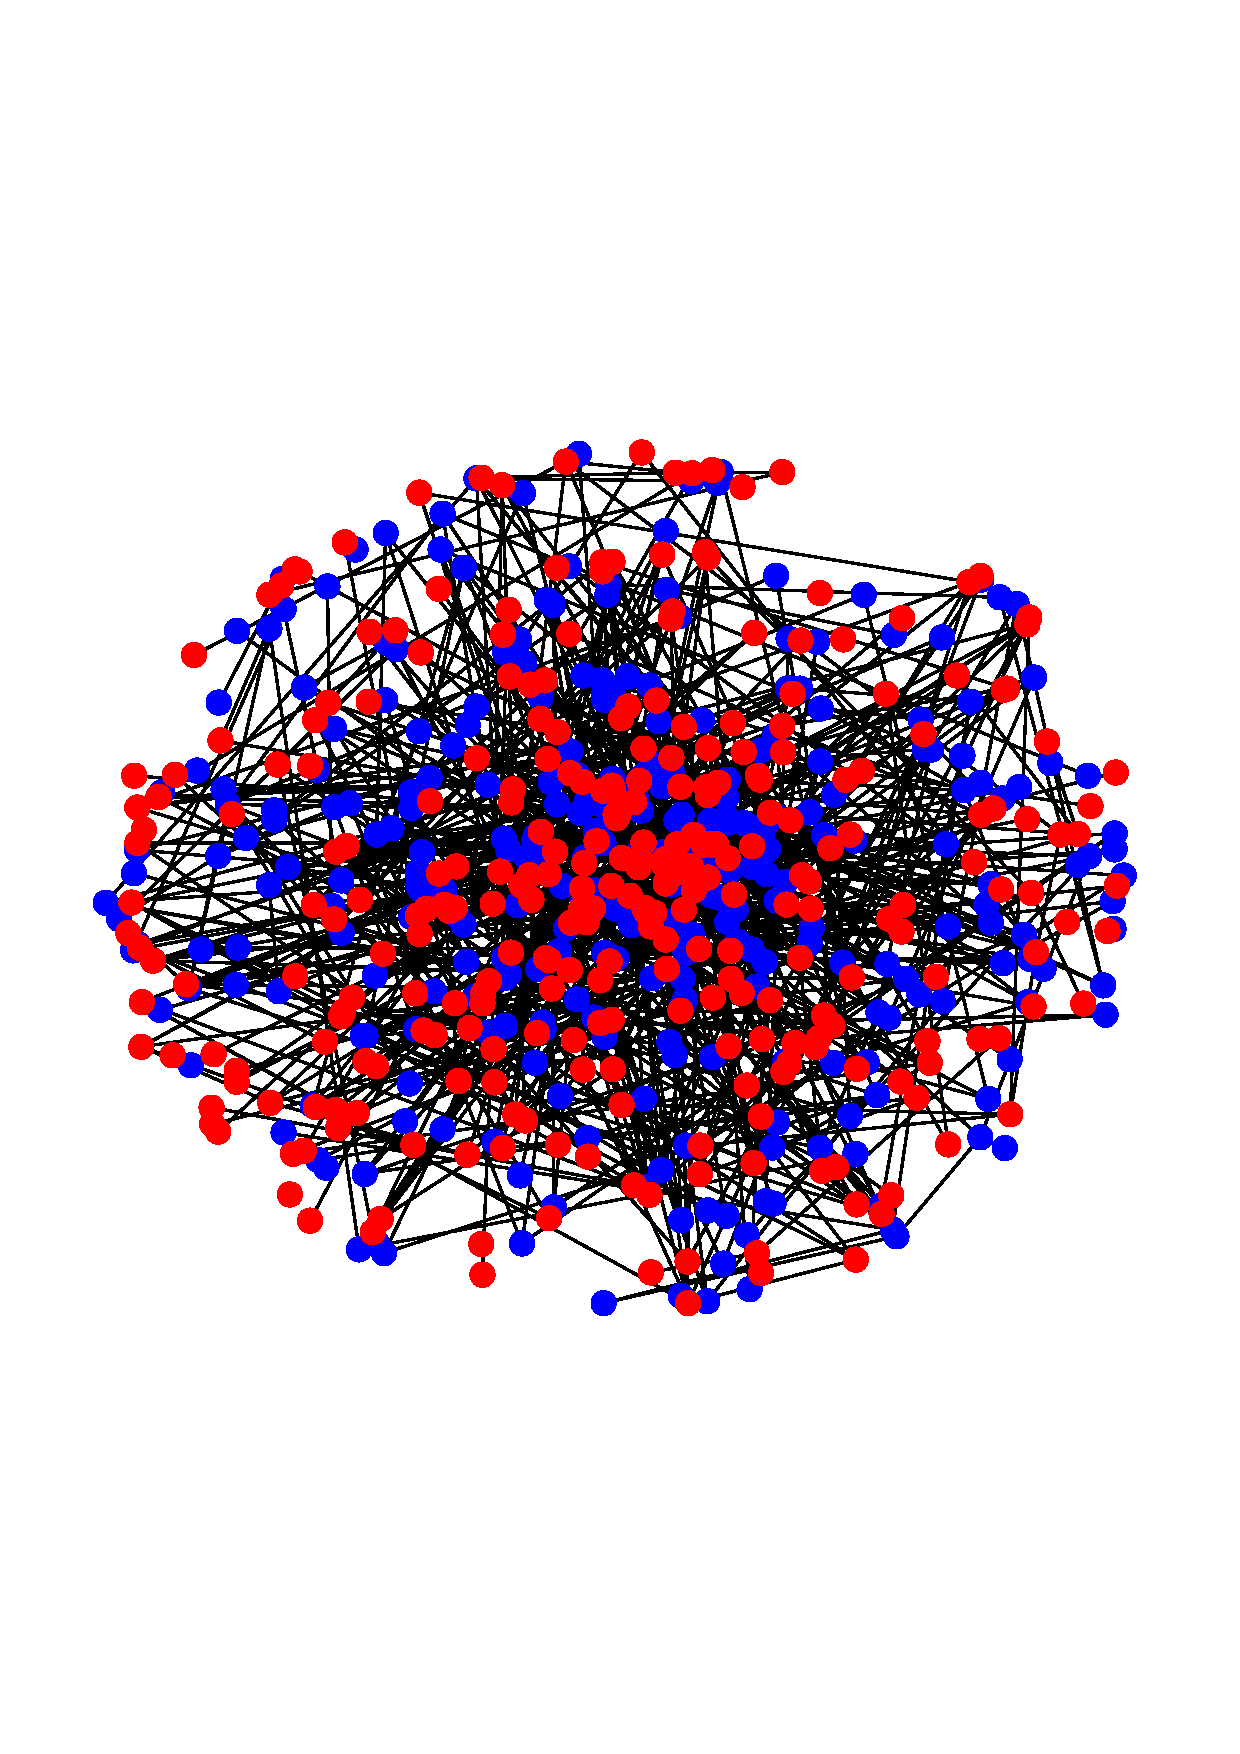
\includegraphics[width=\textwidth]{benno2t.pdf}
		\end{figure}
		\column{0.05\textwidth}
		$\Rightarrow$
		\column{0.5\textwidth}
		\begin{figure}
		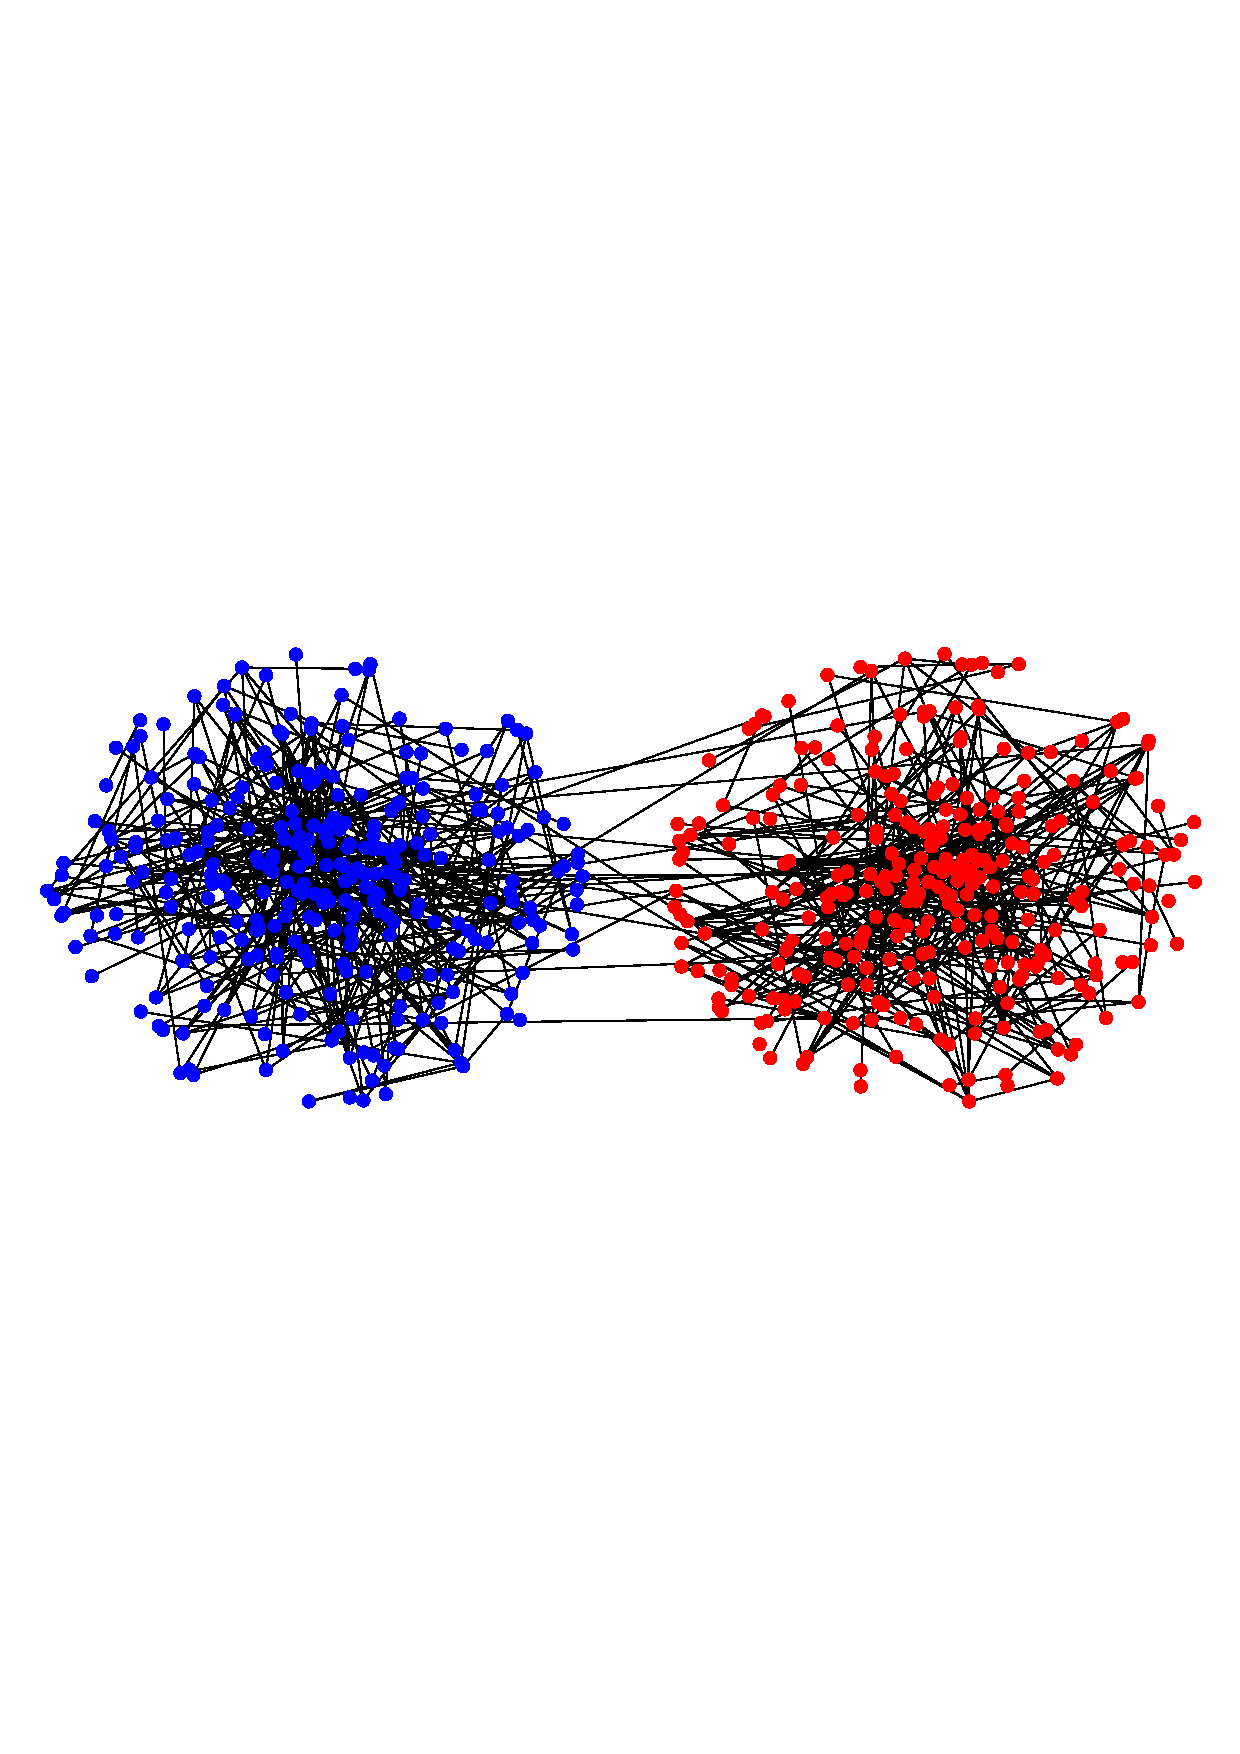
\includegraphics[width=\textwidth]{bennot.pdf}
		\end{figure}
	\end{columns}
\end{frame}


\subsection{Related Work}
\begin{frame}
	\frametitle{Related Work}
\begin{itemize}
\item graph based clustering method
	\begin{enumerate}
		\item \citeauthor{de} in \citeyear{de} proposed a hierarchical density estimate method 
%to do outlier detection
		\item \citeauthor{mac} in \citeyear{mac} proposed a minimum average cost clustering method 
%which shares the same hierarchical clustering structure with info-clustering.
		\item \citeauthor{ic} in \citeyear{ic} proposed info-clustering method
%which is a hierarchical clustering method.
	\end{enumerate}
\item Graph partition algorithm
\begin{enumerate}
\item \citeauthor{psp} in \citeyear{psp} proposed an algorithm to compute the principal sequence of partition 
\item \citeauthor{pmf} in \citeyear{pmf} proposed a parametric algorithm for the same task 
\end{enumerate}
\end{itemize}
Our work
\begin{itemize}
\item Info-Detection method
\item Improved algorithm for principal sequence of partition
\end{itemize}
\end{frame}
\section{Formulation of Info-Detection}
\subsection{Info-Clustering}
\begin{frame}
\frametitle{Review of Info-Clustering}
\begin{enumerate}
\item directed graph $G(V, E)$; Node set $Z_V=\{Z_i | i \in V\}$
\item partition $\P=\{C_1, \dots, C_k\}, \bigcup_{i=1}^k C_i = V$ and $i\neq j \Rightarrow C_i \cap C_j = \emptyset$
\item $\Pi$ is the collection of all partitions of $V$, $\Pi' = \Pi \backslash \{V\}$
\item $f(\cdot)$ is the graph in-cut function, $f(C)=\sum_{i \neq C, j\in C, (i,j) \in E} w_{ij}$
\item $f[\cdot]$ is a function defined on $\Pi$ by $f[\P]=\sum_{C\in \P}f(C)$
\end{enumerate}
\begin{definition}[info-cluster]
Given $G(V, E)$, the cluster set $C_{\gamma}(Z_V)$ is defined as 
\begin{align}
I_{\mathcal{P}}(Z_V) & = \frac{f[\P]}{ \abs{\mathcal{P}} - 1}\\
I(Z_V) & = \min_{\mathcal{P} \in \Pi'(V)} I_{\mathcal{P}}(Z_V) \\
C_{\gamma}(Z_V) & := \textrm{maximal}\{ B \in V \vert \, \abs{B} > 1, I(Z_B) > \gamma \}
\end{align}
\end{definition}
\end{frame}
\begin{frame}{Review of Info-Clustering}
\begin{enumerate}
\item  every two sets $C(Z_V)=\bigcup_{\gamma \geq 0} C_{\gamma}(Z_V)$ are either disjoint or have subset relationship
\item sets from $C(Z_V)$ can be arranged in a clustering tree $\mathcal{T}$; The leaf node of $\mathcal{T}$ is $\{j\}$.
\item the largest threshold value $\gamma_N = \max_{A\subseteq V, \abs{A}>1} I(Z_A)$; The maximal set to achieve this is denoted $B$; $\gamma_N = I(Z_B)$.
\end{enumerate}
Example
\begin{columns}
\column{0.45\textwidth}
\begin{figure}
		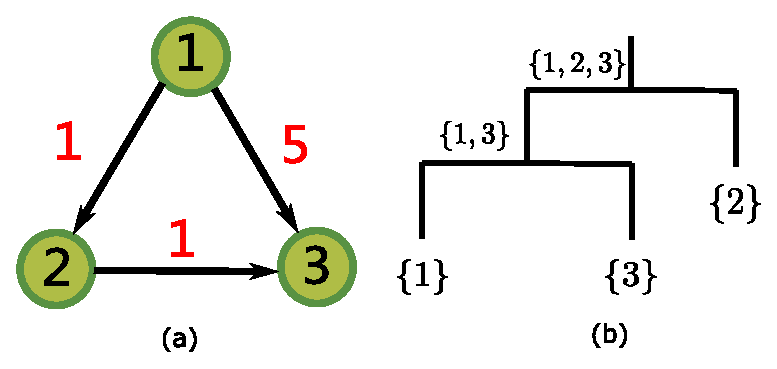
\includegraphics[width=4.5cm]{pic/example_directed.eps}
\end{figure}
\column{0.55\textwidth}
	\begin{equation*}
	C_{\gamma}(Z_V)	=\begin{cases}
					\{\{1,2,3\}\} & \gamma < 2 \\
					\{\{1,3\}\} & 2\leq \gamma < 5 \\
					\emptyset & \gamma \geq \gamma_N = 5
		\end{cases}
	\end{equation*}
\end{columns}
\end{frame}
\subsection{Info-Detection}
\begin{frame}
	\frametitle{Info-Detection Method}
\begin{itemize}
\item For $\gamma_N = I(Z_B)$, nodes in $B$ are inliers and nodes in $V\backslash B$ are outliers.
\item The ourlier score $Z_j$ for $j \in V\backslash B$ is measured with the depth of the set $\{j\}$ in the hierarchical tree.
\end{itemize}
Example
	\begin{figure}
		\centering
		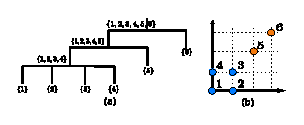
\includegraphics[width=9cm]{pic/outlier_example.eps}
		\caption*{Info-Detection applied to 6 points on Cartesian plane, with $w_{ij} = \exp(-d_{ij}^2)$}\label{fig:ex}
	\end{figure}
\end{frame}
\begin{frame}{Prediction Scheme for Info-Detection}
For newly added node $i'$. Let $V'=B\cup \{i'\}$, we can compute $\gamma'_N$ for $G(V', E(V'))$.
$ \gamma'_N > \gamma_N \iff i'$ is normal observation. We found that
\begin{proposition}
\begin{equation}
\gamma'_N > \gamma_N \iff  \sum_{i \in B} w_{ii'} > \gamma_N 
\end{equation}
\end{proposition}
\begin{figure}
	\centering
	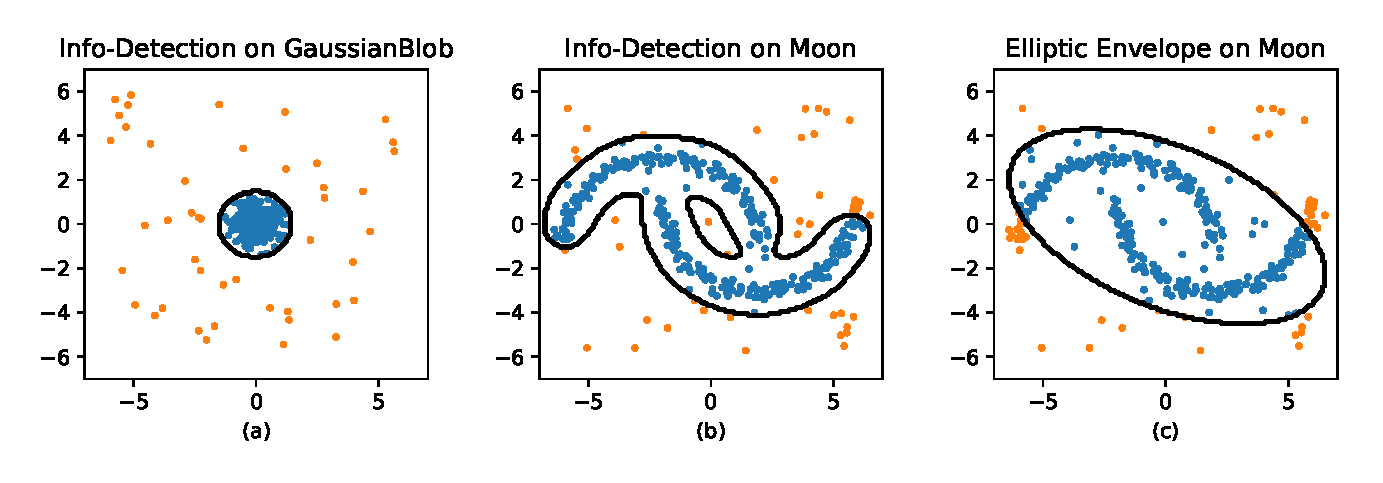
\includegraphics[width=\textwidth]{pic/outlier_boundary_illustration.eps}
	\caption*{Detection boundary lines}	\label{fig:boundary}
\end{figure}
\end{frame}

\subsection{Algorithms}
\frame{\tableofcontents[currentsection]}
\begin{frame}{Review of Principal Sequence of Partition}
It has been found the mathematical structure of info-clustering is the same with that of principal sequence of partition.
\begin{definition}[Principal Sequence of Partition]
\begin{align}
h_{\P}(\lambda) &=  f[\P] - \abs{\P} \lambda  \label{eq:hPL}\\
h(\lambda) &= \min_{\P \in \Pi'(V)} h_{\P}(\lambda) \label{eq:hLambda}
\end{align}
The optimal partitions $\P_1, \dots, \P_k$ for $h(\lambda)$ are nested such that $\P_1 \succeq \P_2 \dots \succeq \P_k$,  which are called principal sequence of partition (PSP) of the graph $G$.
\end{definition}
We call $\lambda^*$ a critical value for PSP if $\P_i, \P_{i+1}$ are both minimizer for $h(\lambda^*)$ in \eqref{eq:hLambda}.
The largest critical value is equal to $\gamma_N$ and the largest set in $\P_{k-1}$ is equal to $B$.
\end{frame}
\begin{frame}
\frametitle{Review of Narayanan's Algorithm to compute PSP}
\begin{columns}
\column{0.5\textwidth}
\algsetup{linenosize=\tiny}
\begin{algorithm}[H]
\caption*{Narayanan's Algorithm}\label{alg:psp}
{\tiny
\begin{algorithmic}[1]
\REQUIRE a directed graph $G(V,E)$
\ENSURE A sorted critical value array \textbf{L} and a reverse ordered array \textbf{PSP} containing $\P_1,\dots, \P_k$.
\STATE \textbf{L}  $\leftarrow$ empty list.
\STATE $Q\leftarrow \{V\}, P \leftarrow \{ \{i \} | i \in V\}$
\STATE $\mathbf{PSP}= [Q, P]$
\STATE \texttt{Split}$(Q,P)$
\STATE sort $L$ and sort $\mathbf{PSP}$ with respect to $\succeq$ 
\FUNCTION{\texttt{Split}$(Q,P)$}
 \STATE\label{alg:gamma} $\gamma' = {1 \over \abs{P} - \abs{Q}} (f(P)-f(Q))$
 \STATE $h' = {1 \over \abs{P} - \abs{Q}}(\abs{P} f(Q) - \abs{Q} f(P))$
 \STATE $(\tilde{h}, P') = \texttt{DT}(f,\gamma')$
 \IF{$\tilde{h} = h'$}
 	\STATE insert $\gamma'$ to $\mathbf{L}$
 \ELSE
 	\STATE insert $P'$ to $\mathbf{PSP}$
 	\STATE \texttt{Split}$(Q, P')$
 	\STATE \texttt{Split}$(P',P)$
 \ENDIF
\ENDFUNCTION
\end{algorithmic}
}
\end{algorithm}
The whole graph $G$ is used in each computation of \texttt{DT} routine.
\column{0.5\textwidth}
Example
\begin{figure}
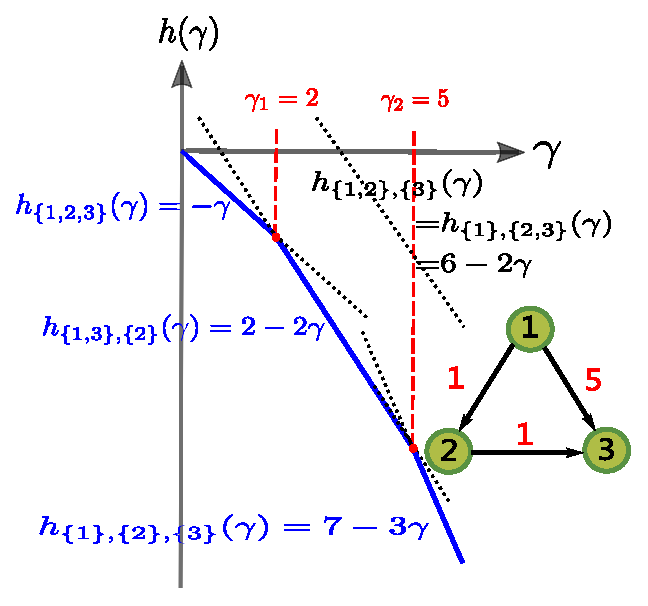
\includegraphics[width=4.5cm]{pic/dt_with_graph.eps}
\end{figure}
\begin{align*}
\P_0  & = \{\{1,2,3\}\} \\
\P_1  & = \{\{1,3\},\{2\}\} \\
\P_2  & = \{\{1\},\{2\},\{3\}\} 
\end{align*}
\end{columns}
\end{frame}
\begin{frame}
\frametitle{Improved PSP Algorithm}
\begin{columns}
\column{0.5\textwidth}
\vskip -1.2em
\algsetup{linenosize=\tiny}
\begin{algorithm}[H]
\caption*{{\footnotesize Improved PSP Algorithm}}
{\tiny
	\begin{algorithmic}[1]
		\REQUIRE a directed graph $G(V, E)$
		\ENSURE a hierarchical tree $\mathcal{T}(K, E)$ where $K \subseteq 2^{V}$ is node set and $E$ is edge set.
		\STATE initialize tree $\mathcal{T}$ with $V$ as root node, $\{j\}(j\leq \abs{V})$ as leaf node and no stem node.
		\STATE \texttt{Split}($G, V$)
		\FUNCTION{\texttt{Split}($\widetilde{G}, \widetilde{V}$)}
		\STATE $w$ is the summation of all edge weights of $\widetilde{G}$ 
		\STATE $\gamma' = \frac{w}{\abs{V(\widetilde{G})}-1}$ where $V(\widetilde{G})$ is node set of graph $\widetilde{G}$ \label{alg:gamma_apostrophe}
		\STATE $(\tilde{h}, P') = \texttt{DT}(\widetilde{G}, \gamma')$ 
		\IF{$\tilde{h} = - \gamma'$}
		\STATE add edge weight $\gamma'$ in $\mathcal{T}$ from $\widetilde{V}$ to its children
		\ELSE
		\FOR{$S$ in $P'$ and $\abs{S}>1$}
		\STATE make children of $\widetilde{V}$ in $\mathcal{T}$ have new parent $S$		
		\STATE make the parent of $S$ be $\widetilde{V}$
		\STATE \texttt{Split}($\widetilde{G}[S], S$) where $\widetilde{G}[S]$ is the subgraph of $\widetilde{G}$ restricted on $S$
		\STATE contract $S$ to a single node in $\widetilde{G}$ % graph \widetilde{G} is modified
		\ENDFOR 
		\STATE \texttt{Split}($\widetilde{G}, \widetilde{V}$)		
		\ENDIF
		\ENDFUNCTION
	\end{algorithmic}
}
\end{algorithm}
\vskip -1.2em
Smaller graph $G$ is used in each computation of \texttt{DT} routine.
\column{0.5\textwidth}
Example
\begin{figure}
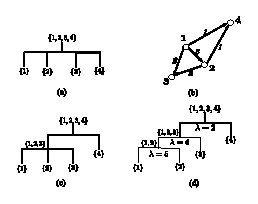
\includegraphics[width=5cm]{pic/alg_illustration.eps}
\end{figure}
Time complexity for dense graph
\begin{itemize}
\item Narayanan's: $O(n^5)$
\item Ours: $O(n^4)$
\end{itemize}
\end{columns}
\end{frame}

\begin{frame}
	\frametitle{Empirical Comparison for three implementation of PSP}
\begin{figure}
	\centering
	\begin{subfigure}{0.4\textwidth}
		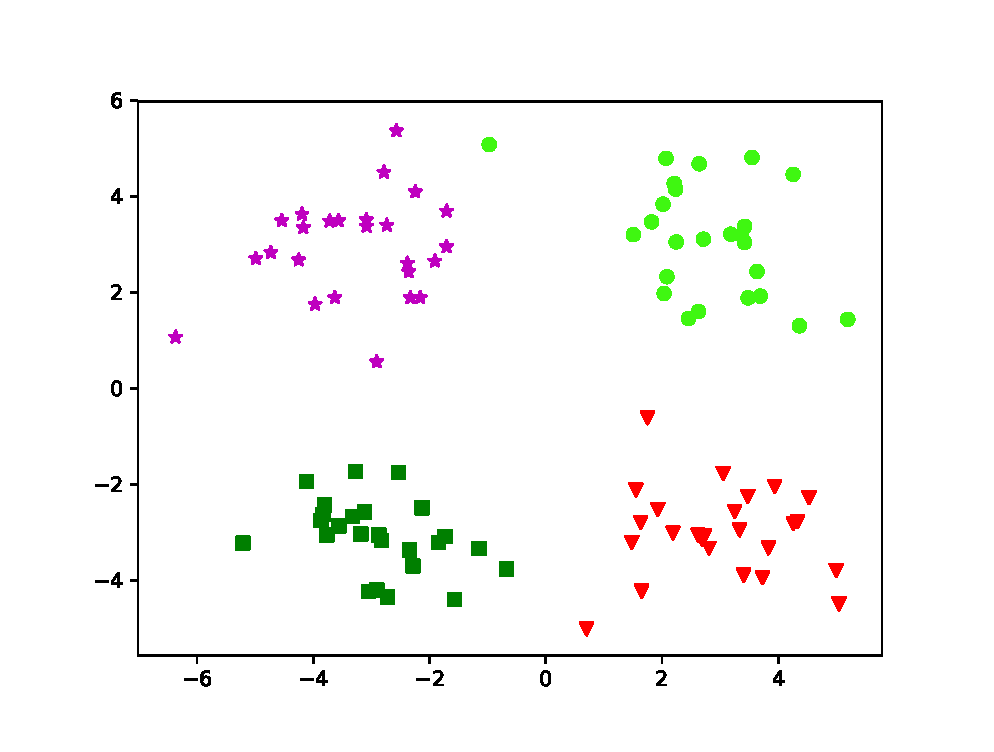
\includegraphics[width=\textwidth]{pic/gaussian-blob-dataset.eps}		
\vskip -1.0em

   \caption*{\quad\quad$\abs{V}=O(\abs{E}^2)$ (above) \\ \quad\quad$\abs{V}=O(\abs{E}^{1.5})$(below)}
	\end{subfigure}~
	\begin{subfigure}{0.4\textwidth}
		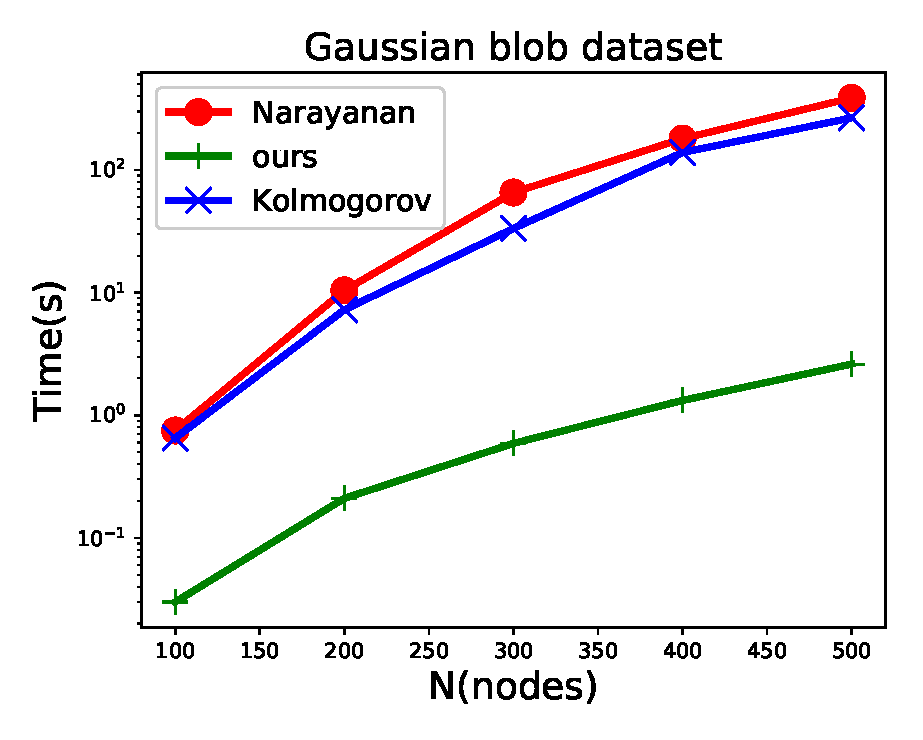
\includegraphics[width=\textwidth]{pic/time_complexity_gaussian.eps}
	\end{subfigure}
\end{figure} 
\begin{figure}
	\centering
\vskip -1.0em
	\begin{subfigure}{0.4\textwidth}
		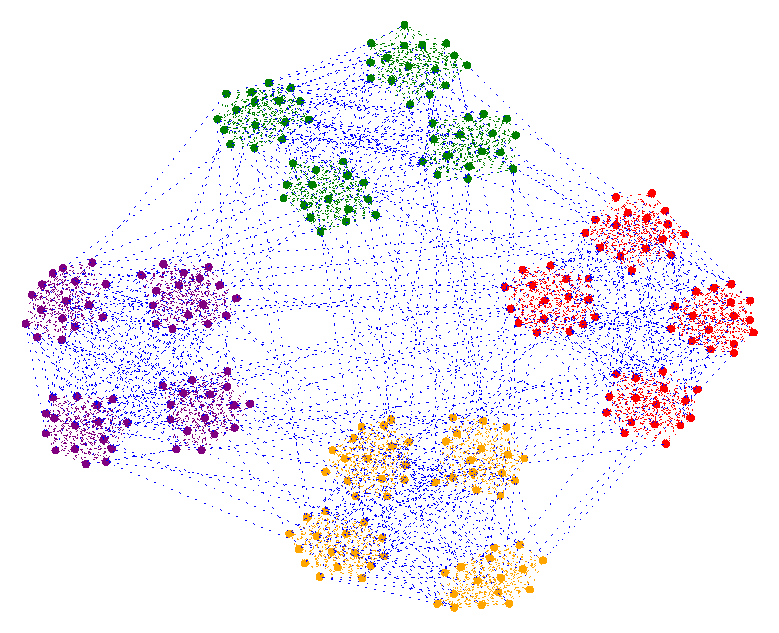
\includegraphics[width=\textwidth]{pic/two_level_new.eps}		
	\end{subfigure}~
	\begin{subfigure}{0.4\textwidth}
		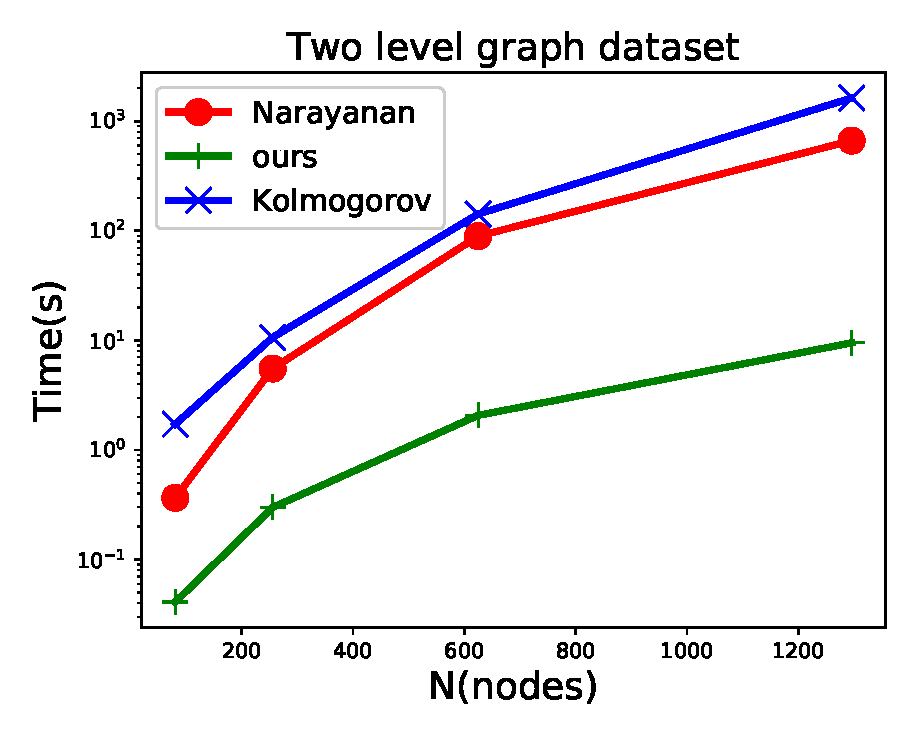
\includegraphics[width=\textwidth]{pic/time_complexity_two_level.eps}
	\end{subfigure}
\end{figure} 
\end{frame}
%\section{Experimental Results}
\begin{frame}
	\frametitle{Experimental Results}
\begin{table}
\centering
\begin{tabular}{ccccc}
\hline
              &  GaussianBlob   &      Moon       &  Lymphography  &     Glass     \\
\hline
   Type    & artificial & artificial & real-world & real-world \\
   N(Inliers) & 255  & 300 & 142  & 207 \\
   N(outliers)   & 45 &  45  & 6 & 7 \\
   N(features)   & 2 &  2  & 19 & 7  \\
\hline
\end{tabular}
\end{table}
\begin{itemize}
\item True Positive Rate (TPR)  $=\frac{N(\textrm{detected inliers})}{N(\textrm{inliners})} \geq 90\% $
\item True Negative Rate (TNR) $=\frac{N(\textrm{detected outliers})}{N(\textrm{outliers})}$
\end{itemize}
\begin{table}
\centering
{\scriptsize
\begin{tabular}{ccccc}
\hline
       TPR/TNR        &  GaussianBlob   &      Moon       &  Lymphography  &     Glass     \\
\hline
    Info-Detection    & 100\%/100\% &  96.7\%/82.2\%  & 97.9\%/100\% & 91.2\%/11.1\% \\
 local outlier factor & 100\%/100\% & 100\%/100\% & 98.6\%/83.3\%  & 96.6\%/22.2\% \\
   isolation forest   & 100\%/100\% &  96.7\%/77.8\%  & 99.3\%/100\% & 90.2\%/22.2\% \\
  elliptic envelope   & 100\%/100\% &  91.3\%/42.2\%  & 93.0\%/83.3\%  & 94.6\%/0.0\%  \\
    one class SVM     &  98.8\%/91.1\%  &  93.0\%/55.6\%  & 93.0\%/66.7\%  & 91.7\%/22.2\% \\
\hline
\end{tabular}
}
\end{table}

\end{frame}	
\section{Conclusion}
\begin{frame}
\frametitle{Conclusion}
\begin{itemize}
\item Formulate Info-Detection method
\item Propose improved principal sequence of partition algorithm 
\item Demonstrate Info-Detection performs well on some datasets
\end{itemize}
\end{frame}
%\section*{Reference}
\begin{frame}
\frametitle{Reference}
\setbeamertemplate{bibliography item}[triangle]
\bibliographystyle{plainnat}
{\footnotesize
\bibliography{id}
}
\end{frame}


\subsection{Ising Model}
\begin{frame}
\frametitle{Ising model}
	\begin{columns}
		\column{5cm}
		\begin{figure}
			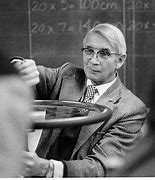
\includegraphics[width=3cm]{ernst_ising.jpeg}
			\caption{Ernst Ising, German physicist}
		\end{figure}
		\column{5cm}
	In statistical physics, Ising model refers to the magnetic spins that can be in one of two states (+1 or -1).
	
	$T_c$: critical temperature.
	
	\end{columns}
\begin{figure}
	\centering
	\begin{subfigure}{0.4\textwidth}
		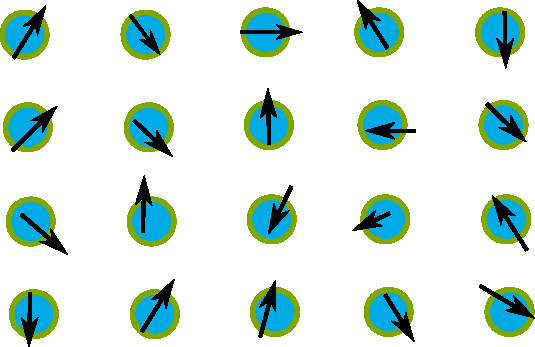
\includegraphics[width=0.7\textwidth]{Tlarge.pdf}
		\caption{$T>T_c$, random spins}
	\end{subfigure}~
	\begin{subfigure}{0.4\textwidth}
		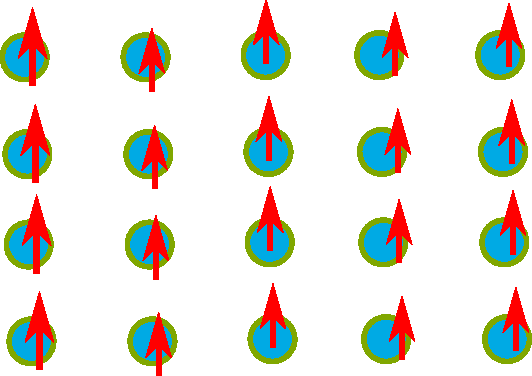
\includegraphics[width=0.65\textwidth]{Tsmall.pdf}
		\caption{$T<T_c$, spins align}
	\end{subfigure}
\end{figure}
\end{frame}

\begin{frame}
\frametitle{Canonical ensemble}
\begin{columns}
	\column{0.5\textwidth}
The distribution of particles:
\begin{equation*}
P(\sigma = \bar{\sigma}) = \frac{1}{Z} \exp(-\beta H(\bar{\sigma}))
\end{equation*}
\begin{itemize}
	\item $Z$: partition function
	\item $\beta$: inverse temperature
	\item $H$: Hamiltonian energy
	\item $\sigma \in \{\pm 1\}^n$: particle state 
\end{itemize}
	\column{0.5\textwidth}
	\begin{tabular}{ccc}
		No & Micro state & Macro state ($H$) \\
		1 & $\uparrow\uparrow\uparrow$ & -3 \\
		2 & $\uparrow\uparrow\downarrow$ & 1 \\
		3 & $\uparrow\downarrow\uparrow$ & 1 \\
		4 & $\downarrow\uparrow\uparrow$ & 1 \\
		5 & $\uparrow\downarrow\downarrow$ & 1 \\
6 & $\downarrow\uparrow\downarrow$ & 1 \\
7 & $\downarrow\downarrow\uparrow$ & 1 \\
8 & $\downarrow\downarrow\downarrow$ & -3 \\
	\end{tabular}
\end{columns}
\begin{block}{Hamiltonian for Ising model}
	Given a graph $G(V, E)$,
	\begin{equation*}
	H(\sigma) = -\sum_{\{i,j\} \in E(G)} \sigma_i \cdot \sigma_j
	\end{equation*}

\end{block}

\end{frame}
\begin{frame}
\frametitle{Square-lattice Ising model}
\begin{block}{spontaneous magnetization}
	% 磁化强度
	$M = \frac{1}{N} \sum_{i=1}^N \sigma_i$: spontaneous magnetization for $N\to \infty$:
	\begin{enumerate}
		\item $T< T_c$, $M>0$, spontaneous magnetization exists;
		\item $T> T_c$, $M=0$, no spontaneous magnetization.
	\end{enumerate}
\end{block}
\begin{figure}
	\centering
	\begin{subfigure}{0.45\textwidth}
		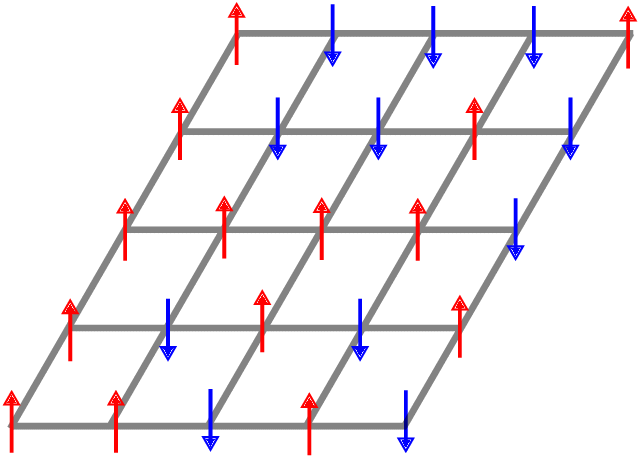
\includegraphics[width=\textwidth]{square-lattice.png}
		\caption{square lattice}
	\end{subfigure}~
	\begin{subfigure}{0.53\textwidth}
		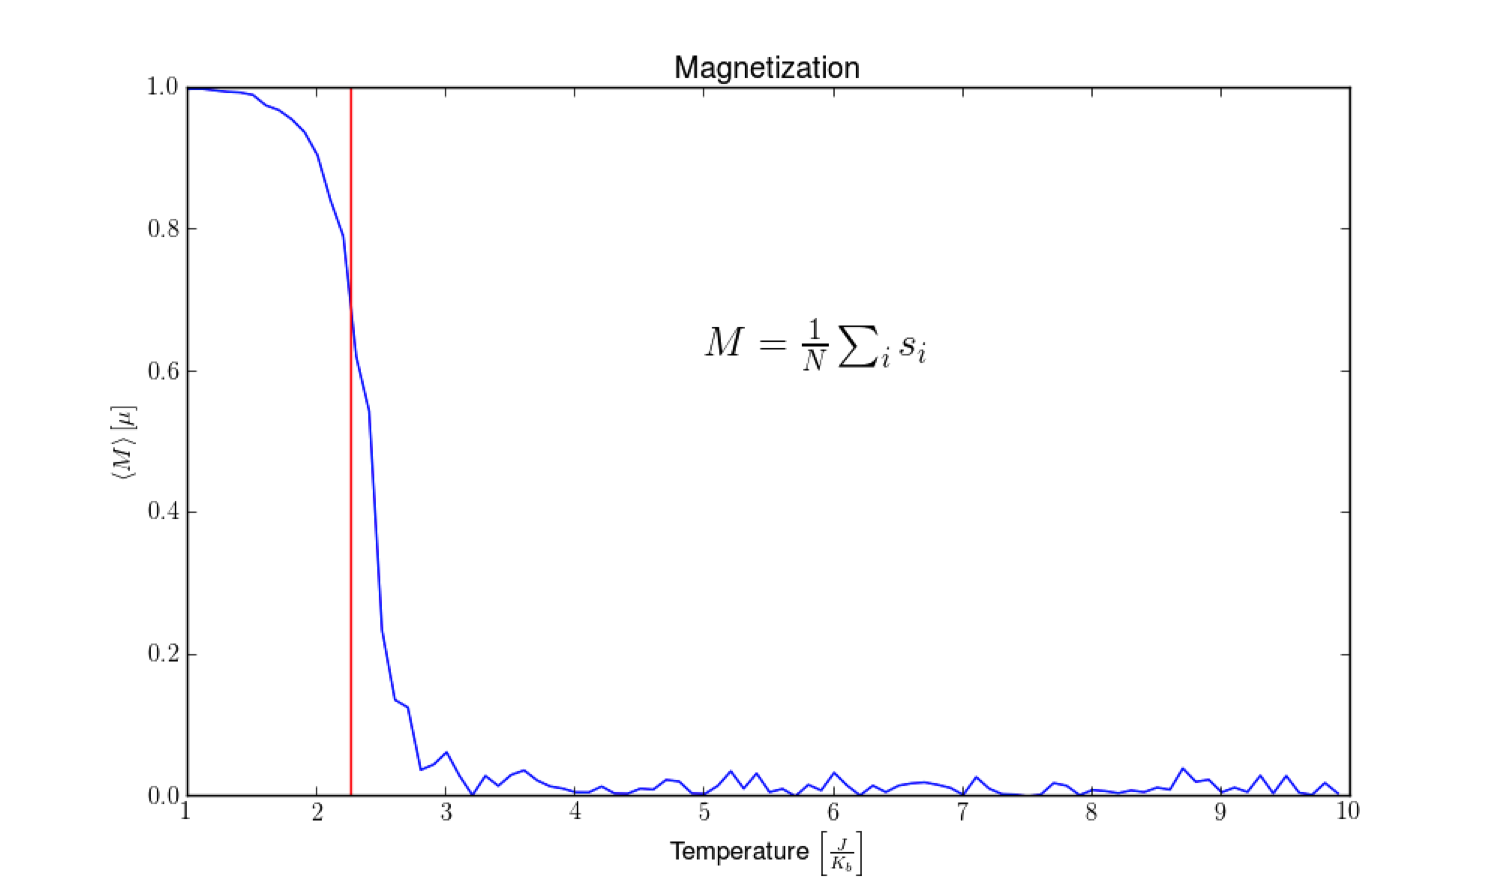
\includegraphics[width=\textwidth]{monte-carlo-ising-6.png}
		\caption{Simulation result}
	\end{subfigure}
\end{figure}

\end{frame}


\begin{frame}
\frametitle{Metropolis algorithm}
\begin{block}{Charateristics}
\begin{itemize}
	\item commonly used to simulate Ising model
	\item single-spin-flip dynamics 
	\item stochastic method for optimization
\end{itemize}
\end{block}
	\begin{algorithmic}[1]
	\STATE random initialize $\bar{\sigma}$
	\STATE randomly choosing a new state $\bar{\sigma}'$ by flipping one spin site
	\STATE compute $\Delta H= H(\bar{\sigma}') - H(\bar{\sigma})$
	\IF{$\Delta H < 0$}
	\STATE $\bar{\sigma} \leftarrow \bar{\sigma}'$
	\ELSE
	\STATE with probability $\exp(-\beta \Delta H)$ 
	such that $\bar{\sigma} \leftarrow -\bar{\sigma}'$ 
	\ENDIF
	\STATE repeat 2-8 until convergence
\end{algorithmic}
\end{frame}

\begin{frame}{Community Detection with Side Information}
	\begin{columns}
		\column{0.5\textwidth}
	\begin{figure}
		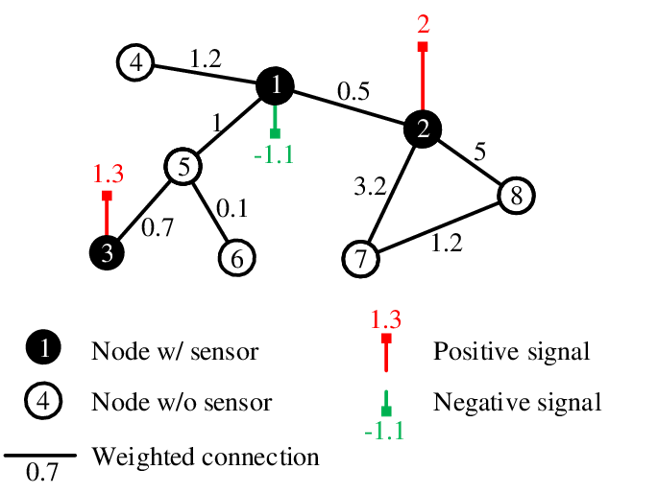
\includegraphics[width=0.8\textwidth]{si.png}
		\caption{\scriptsize Graph Model with Side Information}
	\end{figure}
	\column{0.5\textwidth}
	Incorporating side information in graph model
	can improve the performance of Community Detection
	\begin{block}{Objective}
		Investigate quantitatively how side information influences
		the detection error rate for a specific graph model
	\end{block}
	\end{columns}
\end{frame}
\subsection{Stochastic Block Model}
\begin{frame}{Binary Symmetric Stochastic Block Model}
	\begin{block}{Characteristics}
		\begin{itemize}
		\item a probabilistic model to generate random graph
		\item larger probability for the existence of edges within the same community
		\item smaller probability for the existence of edges between different communities
		\end{itemize}
		\end{block}
		\begin{columns}
			\column{0.33\textwidth}
				\begin{figure}
				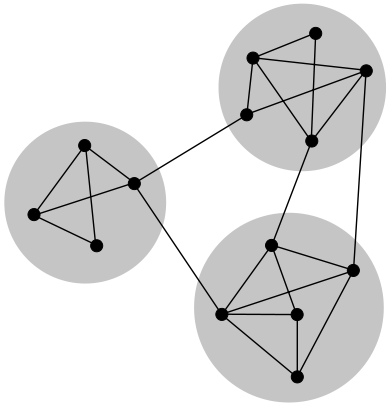
\includegraphics[width=\textwidth]{sbm.png}
			\end{figure}
		\column{0.67\textwidth}
		\quad$(G,Y)\sim \textrm{SSBM}(n, p, q)$
		\begin{itemize}
			\item $Y$: community labels
			\item $n$: the number of nodes
			\item $p$: probability of connecting within clusters
			\item $q$: probability of connecting across clusters
		\end{itemize}
		\end{columns}	
\end{frame}
\begin{frame}{Detection Algorithms and Recovery Metrics}
	\begin{description}
		\item[Observation] random graph $G$, generated by $\textrm{SSBM}(n,p,q)$;
		\item[Estimator] $\hat{Y}(G)$, an algorithm to recover node labels $Y$;
		\item[Error probability] $P_e=P(\hat{Y} \neq \pm Y)$
	\end{description}
	
	\begin{block}{Known Results [Abbe-Bandeira-Hall, 2014]}
		\begin{itemize}
		\item Community labels $Y$ are symmetric: half $+1$, half $-1$;
		\item $p = a\frac{ \log n}{n}, q = b \frac{ \log n}{n}$;
		$\sqrt{a} - \sqrt{b} > \sqrt{2}$
		\item $P_e \to 0$ as $n \to \infty$.
		\end{itemize}
	\end{block}
	\begin{block}{Problem of Error Rate}
	 Does $\lim_{n \to \infty}\frac{\log P_e}{\log n}$
	 exist ?
	\end{block}
\end{frame}
\subsection{Related Works}
\begin{frame}{Related Works}
	% must mention the work of concurrent submission and explain
	% the difference between the two
	\begin{enumerate}
		\item Phase transition study on SBM with side information
		[Saad-Nosratinia, 2018]
		\item Efficient SDP algorithm to achieve exact recovery
		[Sima-Feng, concurrent submission]
		\item Weak recovery error rate in SBM
		[Zahng-Zhou, 2016]
	\end{enumerate}
	\begin{block}{This Work}
		\begin{enumerate}
			\item Optimal error rate study
			\item Does not take implementation of algorithm into consideration
			\item Strong recovery scenario with side information
		\end{enumerate}
	\end{block}
\end{frame}
\begin{frame}
	\frametitle{Phase transition of SBM}
	\begin{block}{Exact Recovery of SBM [1]}
		$P_e=P(\hat{X} \neq \pm X)$: exact recovery for $n \to \infty$
		\begin{enumerate}
			\item $\sqrt{a} - \sqrt{b} > \sqrt{2}$, $P_e \to 0$, there exists algorithms to achieve exact recovery;
			\item $\sqrt{a} - \sqrt{b} < \sqrt{2}$, $P_e \to 1$, no algorithm can achieve exact recovery
		\end{enumerate}
	\end{block}
	{\scriptsize [1]
	Abbe, Emmanuel, Afonso S. Bandeira, and Georgina Hall. "Exact recovery in the stochastic block model." IEEE Transactions on Information Theory 62.1 (2015): 471-487.
	}
	\end{frame}
	
	\section{Stochastic Ising block model}
	\frame{\tableofcontents[currentsection]}
	\begin{frame}
	\frametitle{Stochastic Ising Block Model (SIBM)}
	\begin{itemize}
	\item The Ising model is defined on top of graph generated by SBM.
	\begin{equation*}
	P_{\sigma | G} = \frac{1}{Z} \exp(-\beta H(\bar{\sigma}))
	\end{equation*}
	\item The Hamiltonian energy is compensated by repelling interaction between nodes without edge connection
	\begin{equation*}
	H(\sigma) = \frac{p+q}{2}\sum_{\{i,j\} \not\in E(G)} \sigma_i \cdot \sigma_j - \sum_{\{i,j\} \in E(G)} \sigma_i \cdot \sigma_j
	\end{equation*}
	\end{itemize}
	\begin{description}
		\item[Observation] random graph $G$, generated by $\textrm{SBM}(n,p,q)$;
		\item[Estimator] $\hat{X}^*$, generated by SIBM
		\item[Error Probability] $P_e=P(\hat{X} \neq \pm X) = ?$
	\end{description}
	\end{frame}
	
	\begin{frame}
	\frametitle{Phase transition of SIBM}
	\begin{block}{Assumptions}
		\begin{itemize}
			\item Community labels $X$ are symmetric: half $+1$, half $-1$;
			\item $p = a\frac{ \log n}{n}, q = b \frac{ \log n}{n}$;
			\item $n \to \infty$.
		\end{itemize}
	\end{block}
	\begin{block}{Exact Recovery of SBM by $\hat{X}^*$}
		$P_e=P(\hat{X} \neq \pm X)$: exact recovery for $n \to \infty$
	\begin{enumerate}
		\item $\beta > \beta^*$, $P_e \to 0$, there exists algorithms to achieve exact recovery;
		\item $\beta < \beta^*$, $P_e \to 1$, no algorithm can achieve exact recovery
	\end{enumerate}
	where
	\begin{equation*}
	\beta^* = \frac{1}{2} \log \frac{a+b-2 - \sqrt{(a+b-2)^2-4ab}}{2b}
	\end{equation*}
	\end{block}
	
	\end{frame}
	
	\begin{frame}
	\frametitle{Metropolis algorithm}
	Metropolis algorithm is used to approximate $\hat{X}^*$
	
	
	\begin{figure}
		\centering
		\begin{subfigure}{0.45\textwidth}
			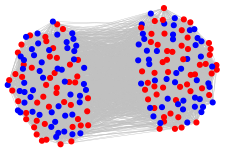
\includegraphics[width=\textwidth]{000.png}
			\caption{Initial label for $\textrm{SBM}(300, 16, 4)$}
		\end{subfigure}~
		\begin{subfigure}{0.53\textwidth}
			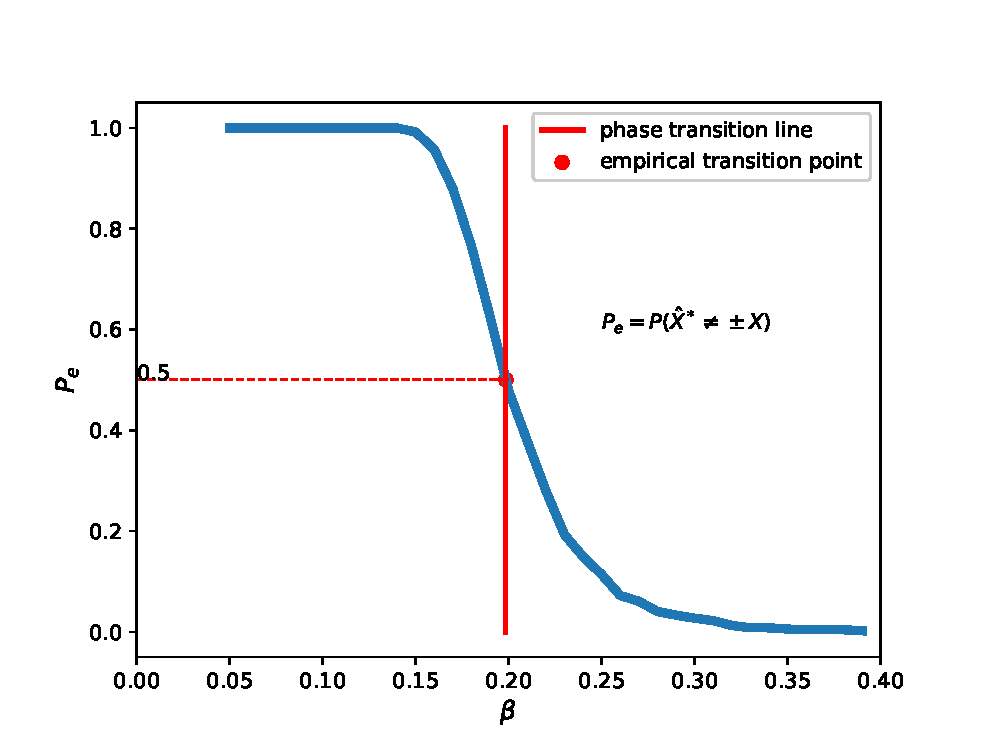
\includegraphics[width=\textwidth]{beta_trans-2020-11-28.eps}
			\caption{$\textrm{SBM}(9000, 16, 4), \beta^*=0.198$}
		\end{subfigure}
	\end{figure}
	\end{frame}
	
	
	
	%\section{Conclusion}
	\begin{frame}
	\frametitle{Conclusion}
	On-going work:
	\begin{itemize}
	\item Extension of SIBM to multiple community case;
	\item connection with other community detection method is explored
	\end{itemize}
	\begin{figure}
		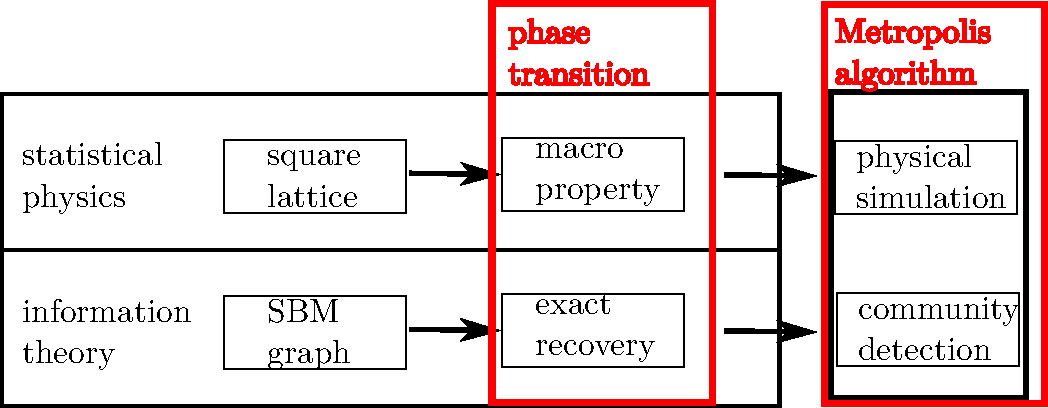
\includegraphics[width=0.8\textwidth]{overview.pdf}
		\caption{Connection between different parts}
	\end{figure}
	\end{frame}
\section{Problem Formulation}
\begin{frame}
\frametitle{Binary Symmetric SBM with Side Information}
\begin{block}{Characteristics of SBMSI}
\begin{itemize}
	\item   Each node includes $m$ additional observations with
	finite-cardinality alphabet.
	\begin{equation*}
		x_{i1}, x_{i2}, \dots, x_{im} \in \{1, 2, \dots, |\mathcal{X}|\}
	\end{equation*}
	\item The observations $X_i$ at $i$-th node are sampled from distribution $P_0$
	or $P_1$ depending on the node label $Y_i$.
	\begin{equation*}
		X_{i1}, X_{i2}, \dots, X_{im} \textrm{ i.i.d. } \sim P_0 \textrm{ or } P_1
	\end{equation*}
	\item $X$ are conditionally independent of the random
	graph $G$.
	\begin{equation*}
		P(G, X | Y) = P(G | Y) P(X | Y)
	\end{equation*}
\end{itemize}
\end{block}

\end{frame}
\begin{frame}\frametitle{Exact Recovery Error Rate}
\begin{block}{Maximum Likelihood}
\begin{itemize}
	\item Theoretically optimal recovery method
	\begin{align*}
		\hat{Y} &= \arg\max_y\ \Pr(x,G|Y=y) \notag \\
		\textrm{s.t.} \ & y_i \in \{\pm 1\}, \sum_{i=1}^n y_i=0 \label{eq:mle}
	\end{align*}
	\item Achieves the optimal error rate $P_e=P(\hat{Y} \neq Y)$
\end{itemize}
\end{block}
Recall: Rényi divergence with order $\frac{1}{2}$:
\begin{equation*}
	D_{1/2}(p_0 || p_1) = -2\log(\sum_{x \in \mathcal{X}} \sqrt{p_0(x)p_1(x)} )
\end{equation*}
\end{frame}
\section{Main Results}
\begin{frame}{Optimal Error Rate for SBMSI}
\begin{enumerate}
	\item Dense Case: $\gamma=\frac{m}{n}, p, q$ are constants
		\begin{equation*}
		-\lim_{n\to \infty} \frac{1}{n}\log P_e =  \gamma D_{1/2}(p_0 || p_1) + D_{1/2}(\Bern(p)||\Bern(q))
		\end{equation*}
	\item Sparse Case: $\gamma=\frac{m}{ \log n},
	a=\frac{np}{\log n}, b=\frac{nq}{\log n}$ are constants
		\begin{equation*}\label{eq:PeMainL}
		-\lim_{n\to \infty}\frac{\log P_e}{\log n}=\gamma D_{1/2}(p_0||p_1) + (\sqrt{a} - \sqrt{b})^2-2
		\end{equation*}
		as long as
		\begin{align*}
			(\sqrt{a}-\sqrt{b})^2-2 
			> 3a^{1/3}b^{1/3}(a^{1/6}-b^{1/6})^2\label{eq:oneC}
		\end{align*}	
\end{enumerate}
\end{frame}
\begin{frame}
\frametitle{Discussion of Main Results}
\begin{enumerate}
	\item SBM with no side information: $\gamma = 0$, $P_e$ decays like $n^{2-(\sqrt{a} - \sqrt{b})^2}$
	\item Connection with Hypothesis Testing Problem and Gärtner Ellis Theorem
	\item Can we remove the additional condition?
	$(\sqrt{a}-\sqrt{b})^2-2 
	> 3a^{1/3}b^{1/3}(a^{1/6}-b^{1/6})^2$
	% This condition is used to control the error
	% of two pairs is smaller than that of one pair in order.
	\item Main results different from the phase transition solution,
	which is the Chernoff information
	between $\textrm{Pois}(\frac{a}{2},\frac{b}{2})\times P_0$ and $\textrm{Pois}(\frac{b}{2}, \frac{a}{2})\times P_1$
	[Asadi-Abbe-Verdú,2017]
\end{enumerate}

\end{frame}
%\section{Sketch of Proof}

\section{Conclusion}
\begin{frame}
\frametitle{Conclusion}
\begin{itemize}
\item The detection error can be
characterized by Rényi divergence and the parameters of SBM
\item Our result provides insight on the
number of features and nodes needed for community
detection task.
\end{itemize}
\end{frame}

\begin{frame}
\frametitle{}
\begin{block}{}
\centering
{\Huge Questions and Answers}
\end{block}
\end{frame}
\end{document}
